\section{...}

We will examine the so-called total domatic number of graphs.
Let $G = (V, E)$ be a graph without isolated vertices.

\begin{definition}
  $S \subseteq V$ is a total dominating set if every vertex has a neighbor in
  $S$. The total domatic number of $G$ is the maximum number of disjoint total
  dominating sets.
\end{definition}

Sometimes it's more convenient to look at total dominating sets as color classes.

\begin{definition}
  A coloring of the vertices is called a $k$-coupon coloring if every vertex
  has a neighbor from each color class. The coupon coloring number of $G$ is
  the maximum $k$ for which a $k$-coupon coloring exists. The coupon coloring
  number is denoted by $\chi_c(G)$.
\end{definition}

It turns out that determining the total domatic number (or equivalently the
coupon coloring number) of a graph is rather hard.

\begin{definition}
  NAE-3SAT ...
\end{definition}

\begin{thm}
  NAE-3SAT is NP-complete.
\end{thm}

\begin{proof}
  ...
\end{proof}

\begin{thm}
  It's NP-complete to decide whether the total domatic number of
  a graph is at least $2$.
\end{thm}

\begin{proof}
  Given a partition of the vertices into $2$ sets, it can be checked in polynomial
  time whether these sets are total dominating sets. So the problem is a member
  of NP.

  For proving NP-completeness, we will show that NAE-3SAT is reducible to this problem
  in polynomial time. Let $C$ be the set of clauses and $X$ be the set of variables
  in an instance of NAE-3SAT. We can assume that every variable $x$ appears in at least
  one clause. Otherwise we add a new clause containing $x$ and $\bar{x}$ to
  the formula. Now we construct the corresponding graph $G$. For each variable $x$,
  introduce $3$ vertices $x_1, x_2, x_3$, and $2$ edges $x_1x_2, x_2x_3$. For each
  clause $c$, introduce a vertex $c$. If $x$ is a literal in $c$, then add the edge
  $cx_1$ to the graph. If $\bar{x}$ is a literal in $c$, then add the edge $cx_3$.

  Suppose $G$ has a partition into $2$ disjoint total dominating sets: $T$ and $F$.
  Assign the value true for each variable $x$ with $x_1 \in T$ and assign the value
  false otherwise. For any variable $x$, $x_1$ and $x_3$ are the only neighbors
  of $x_2$, so $x_1$ and $x_3$ must be in different sets of the partition. If $c$
  is a vertex corresponding to a clause, then it must have neighbors both in $T$
  and $F$, and so the literals in $c$ can't be all true nor false.

  Suppose now that the variables have a truth assignment such that each clause
  contains both true and false literals. Define $T$ and $F$ as follows. Put all
  the vertices corresponding to clauses into $T$. For each variable $x$ put $x_2$
  into $F$. Furthermore, if true was assigned to $x$, then put $x_1$ into $T$, $x_3$
  into $F$, and conversely otherwise.
\end{proof}

Let us note that the constructed graph in the proof is always a bipartite
graph.

\begin{cor}
  It's NP-complete to decide whether the total domatic number of
  a bipartite graph is at least $2$.
\end{cor}


\section{Degree restrictions}

A natural question is whether graphs with an appropriately big minimum degree
always have a total domatic number of at least $2$.

\begin{thm}
  For every $d$ there exists a graph with minimum degree $d$ and without $2$
  disjoint total dominating sets.
\end{thm}
\begin{proof}
  ...
\end{proof}

...Other degree stuff (k-regular, maxdeg-mindeg small enough)...

\section{A conjecture of Goddard and Henning}

From now on we will focus on $2$-coupon colorings and planar graphs. A
conjecture of Goddard and Henning is the following.

\begin{conj}
  If $G$ is a simple triangulated planar graph of order at least $4$, then the
  total domatic number of $G$ is at least $2$.
\end{conj}

stacked graphs...

\begin{remark}
  The simplicity of the graph is necessary. Suppose the graph below has a
  $2$-coupon coloring. Then $A$ and $C$ must have different colors, because
  they are the only neighbors of $B$. Similarly, $C$ and $E$ must have different
  colors, as well as $E$ and $A$. That's a contradiction, since $A$, $C$ and
  $E$ form a triangular.
\end{remark}

\begin{figure}[h]
  \centering
  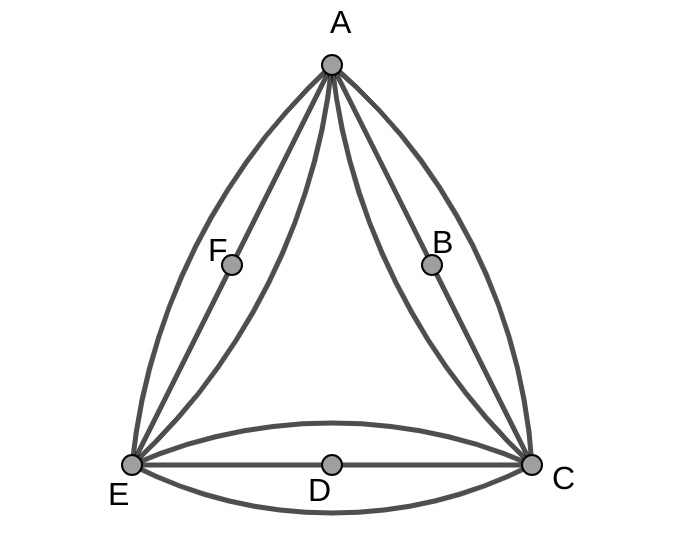
\includegraphics[width=70mm]{parallel}
\end{figure}

\begin{remark}
  Allowing triangulated disks (i.e. planar graphs with at most one face greater
  than $3$), the conjecture doesn't hold. For example, the graph below doesn't
  have a $2$-coupon coloring from similar reasons as the previous one. We will
  show later that this graph is a member of a bigger graph family without $2$
  disjoint dominating sets.
\end{remark}

\begin{figure}[h]
  \centering
  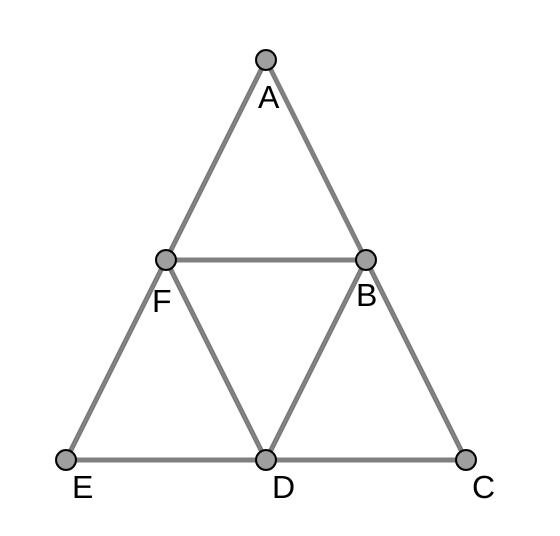
\includegraphics[width=70mm]{sungraph}
\end{figure}

\begin{thm}
  Let $G$ be a triangulated planar graph. If all the vertices of $G$ have an
  odd degree, then there exists a coupon coloring with $2$ colors.
\end{thm}
\begin{proof}
  ...
\end{proof}

\begin{thm}
  Outerplanar graphs ...
\end{thm}

\begin{thm}
  Every triangulated graph with a Hamiltonian circle admits 2 disjoint
  dominating sets.
\end{thm}

Hypergraph connection...
